\section{Registrazione} {

Per accedere ai servizi, gratuiti e accessibili da chiunque, della piattaforma \platform{} è necessario accedere all'applicazione al link riportato qui sotto e, dopo il redirect automatico, scegliere l'opzione di ``Sign up''.

\begin{center}
    \textbf{\url{https://d18v2wlpbu3jpw.cloudfront.net/}}
\end{center}

La registrazione permette di creare un account personale al quale verrà illustrata una guida sotto forma di mappa o lista con i luoghi più apprezzati dai clienti e 
inoltre è possibile iniziare a seguire dei nuovi profili Instagram. \aCapo
Per effettuare la registrazione sulla piattaforma \platform{} è necessario procedere come spiegato di seguito: \aCapo 
Inizialmente apparirà la finestra per effettuare il login, quindi bisognerà premere il link con scritto ``\textbf{Sign Up}''.
\begin{figure}[H]
    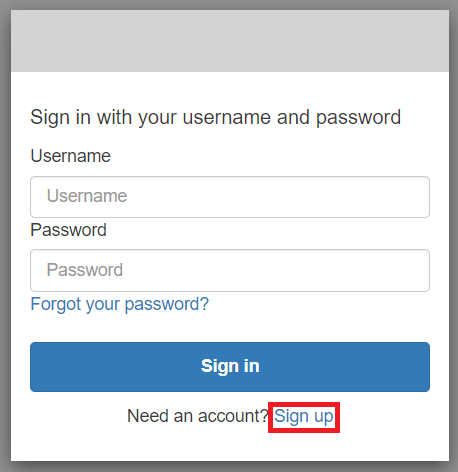
\includegraphics[width=8cm]{sezioni/images/tasto-reg.png}
    \centering
    \caption{Locazione link per la registrazione}
\end{figure}

Dopo aver cliccato sul bottone, si viene reindirizzati in una pagina nuova, contente il seguente form, nel quale verranno inseriti i dati necessari per completare 
correttamente tale passaggio. \aCapo
I dati richiesti sono i seguenti:
\begin{itemize}
    \item Username;
    \item Email;
    \item Password.
\end{itemize}
\begin{figure}[H]
    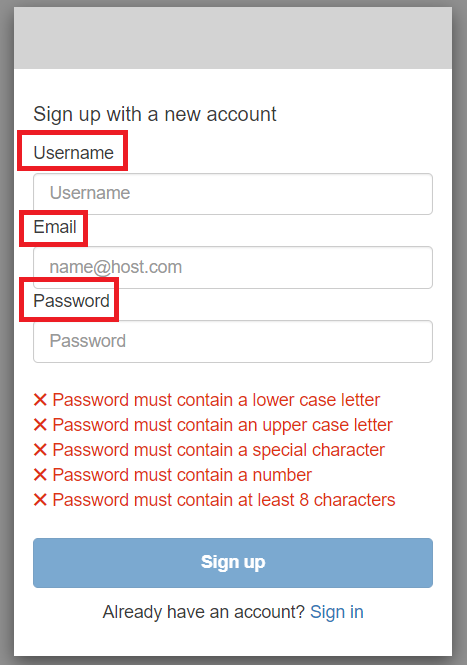
\includegraphics[width=8cm]{sezioni/images/form-reg.png}
    \centering
    \caption{Campi del form per la registrazione}
\end{figure} 

Quando tutti i campi sono stati compilati bisogna cliccare il pulsante con il testo ``Sign up''. 
\begin{figure}[H]
    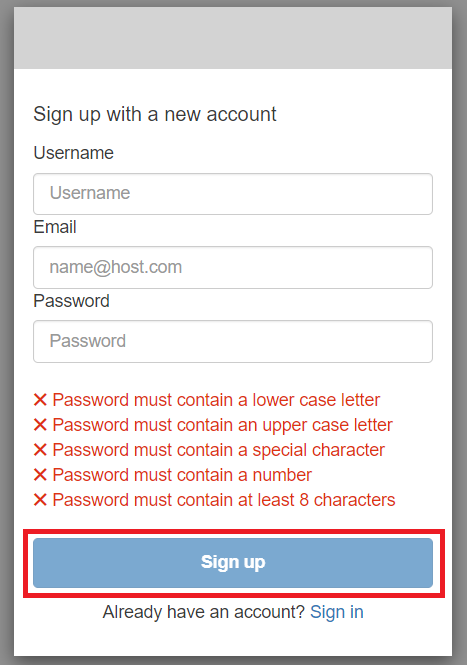
\includegraphics[width=8cm]{sezioni/images/tasto-conf-reg.png}
    \centering
    \caption{Bottone per confermare la registrazione}
\end{figure} 
Dopo aver eseguito questa parte, verrà inviato un codice alla mail indicata durante la compilazione del form: quindi per poter verificare
l'account è necessario riportare nell'apposito spazio il codice e successivamente premere il bottone ``\textbf{Confirm Account}'' 
\begin{figure}[H]
    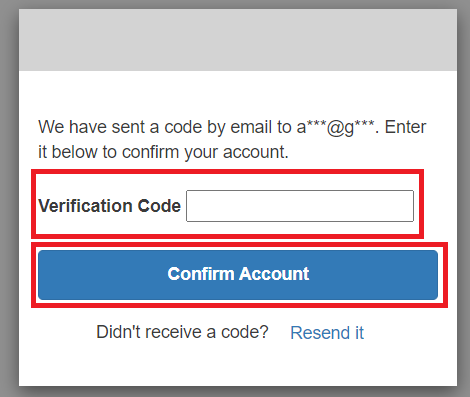
\includegraphics[width=8cm]{sezioni/images/codice-reg.png}
    \centering
    \caption{Codice di conferma account per la registrazione}
\end{figure}

\subsection{Inserimento dati errati} {
L'utente non è in grado di premere il pulsante ``Sign up'' se lascia vuoto anche solo uno spazio dei 3.

    \subsubsection{Formato email errata} {
        Nel campo ``Email'' verrà effettuato un controllo per assicurarsi che il formato mail inserito sia corretto.
        Infatti verrà controllata la presenza del carattere speciale ``@'' e che dopo di essa sia presente del testo.
    }
    
    \subsubsection{Formato password non valida} {
        Come si può notare dalla foto precedente, la password deve rispettare delle specifiche, ovvero:
        \begin{itemize}
            \item Deve contenere un carattere in minuscolo;
            \item Deve contenere un carattere in maiuscolo;
            \item Deve contenere un carattere speciale;
            \item Deve contenere un numero;
            \item Deve contenere minimo 8 caratteri.
        \end{itemize}
    }
}


}
